\title[Soft switching]{Soft switching without resonance}
\section{Soft switching}

\begin{frame}[plain]
	\titlepage
\end{frame}

%%%%%%%%%%%%%%%%%%%%%%%%%%%%%%%%%%%%%%%%%%%%%%%%%%%%%%%%%%%%%
%% Overview %%
%%%%%%%%%%%%%%%%%%%%%%%%%%%%%%%%%%%%%%%%%%%%%%%%%%%%%%%%%%%%%
\subsection{ZVS of a half-bridge}

\begin{frame}
	\frametitle{Overview}
	L2: every hard turn-on of a half-bridge costs $Q_\mathrm{oss}V_\mathrm{DC}$; only zero-voltage switching (ZVS) removes it. Today: ZVS in PWM converters, without a resonant tank.
	\begin{itemize}
		\item The ZVS transition: current, charge and energy
		\item Partial ZVS and the dead-time window
		\item Triangular current mode, active-clamp flyback, phase-shifted full bridge, dual active bridge
		\item Auxiliary circuits and resonant switches
		\item Modelling soft-switched converters; a ZVS design checklist
	\end{itemize}
	After this lecture you can check whether a converter keeps ZVS over its operating range, and size dead time, inductor and negative current for it.
\end{frame}

%%%%%%%%%%%%%%%%%%%%%%%%%%%%%%%%%%%%%%%%%%%%%%%%%%%%%%%%%%%%%
%% ZVS transition %%
%%%%%%%%%%%%%%%%%%%%%%%%%%%%%%%%%%%%%%%%%%%%%%%%%%%%%%%%%%%%%
\begin{frame}
	\frametitle{The ZVS transition}
	\begin{columns}[T]
		\begin{column}{0.42\textwidth}
			\begin{figure}
				\centering
				\begin{circuitikz}[scale=0.76, transform shape]
					\draw (0,0) to[V, l=$V_\mathrm{DC}$] (0,4) -- (2,4);
					\draw (2,4) to[C, l_=$C_\mathrm{oss}$] (2,2) to[C, l_=$C_\mathrm{oss}$] (2,0);
					\draw (2,4) -- (3.2,4) node[nigfete, anchor=D] (HS) {};
					\draw (0,0) -- (3.2,0) node[nigfete, anchor=S] (LS) {};
					\draw (HS.S) -- (LS.D);
					\draw (2,2) -- (3.2,2) node[circ]{};
					\draw (3.2,2) to[short, i=$i_L$] (4.0,2) to[L, l=$L$] (5.8,2);
					\draw (3.2,0) -- (5.8,0) to[V, l_=$V_x$] (5.8,2);
					\draw (1,0) node[ground]{};
					\node[anchor=south east, inner sep=1pt] at (3.15,2.05) {$v_\mathrm{sw}$};
				\end{circuitikz}
				\caption{Half-bridge during the dead time; the inductor ends at a fixed voltage $V_x$}
			\end{figure}
		\end{column}
		\begin{column}{0.55\textwidth}
			\small
			Both switches are off. The inductor current charges one $C_\mathrm{oss}$ and discharges the other. ZVS needs three things:
			\begin{enumerate}
				\item \textbf{Direction}: the current must drive the switch node towards the switch that turns on next.
				\item \textbf{Charge}: $2Q_\mathrm{oss}(V_\mathrm{DC})$ must flow within the dead time. With a stiff current $I$: $t_\mathrm{tr}=2Q_\mathrm{oss}/I$ (L2).
				\item \textbf{Energy}: if the inductor is small, its current falls during the transition. It must not reach zero before the node has arrived.
			\end{enumerate}
			Transformer and winding capacitances add to the charge (L7).
		\end{column}
	\end{columns}
	\blfootnote{Sources: Erickson and Maksimovi\'c, 3rd ed., 2020, Ch.\ 23; Everts et al., IEEE ECCE 2013.}
\end{frame}

%%%%%%%%%%%%%%%%%%%%%%%%%%%%%%%%%%%%%%%%%%%%%%%%%%%%%%%%%%%%%
%% Energy for the transition %%
%%%%%%%%%%%%%%%%%%%%%%%%%%%%%%%%%%%%%%%%%%%%%%%%%%%%%%%%%%%%%
\begin{frame}
	\frametitle{Energy for the transition}
	\begin{columns}[T]
		\begin{column}{0.5\textwidth}
			\footnotesize
			The switch node moves from 0 to $V=V_\mathrm{DC}$; the other end of the inductor sits at $V_x$. With $C$ the output capacitance of each switch, the inductor delivers $i=\left[C(v)+C(V-v)\right]\mathrm{d}v/\mathrm{d}t$ into the node:
			\begin{align*}
				W & =\int(v-V_x)\,i\,\mathrm{d}t                       \\
				  & =\int_0^V(v-V_x)\left[C(v)+C(V-v)\right]\mathrm{d}v \\
				  & =Q_\mathrm{oss}(V)\cdot(V-2V_x)
			\end{align*}
			The energy taken from the inductor depends only on $Q_\mathrm{oss}$, not on the shape of $C_\mathrm{oss}(v)$.
		\end{column}
		\begin{column}{0.47\textwidth}
			\footnotesize
			\begin{itemize}
				\item $V_x=0$: $W=Q_\mathrm{oss}V$, more than the $2E_\mathrm{oss}$ of an energy-equivalent estimate. GaN of L2 at 48\,V: 1.2\,$\mu$J instead of 0.9\,$\mu$J.
				\item $V_x=V/2$ (LLC, DAB with a midpoint): $W=0$. Only the charge, i.e.\ the time, limits ZVS.
				\item Buck 48\,V to 12\,V, high-side turn-on: $W=Q_\mathrm{oss}\cdot24$\,V.
				\item Condition for ZVS, with the current $I_0$ at the start of the dead time: $\frac{1}{2}LI_0^2\geq Q_\mathrm{oss}(V-2V_x)$.
			\end{itemize}
		\end{column}
	\end{columns}
	\blfootnote{Sources: charge-based ZVS analysis, Everts et al., IEEE ECCE 2013; L2.}
\end{frame}

%%%%%%%%%%%%%%%%%%%%%%%%%%%%%%%%%%%%%%%%%%%%%%%%%%%%%%%%%%%%%
%% Task: dead time and energy %%
%%%%%%%%%%%%%%%%%%%%%%%%%%%%%%%%%%%%%%%%%%%%%%%%%%%%%%%%%%%%%
% Two pages: task (page 1) and task with solution (page 2).
\begin{frame}<handout:1-2>
	\frametitle{Dead time and energy}
	\begin{block}{Task (4 minutes)}
		A 48\,V half-bridge uses transistors with $Q_\mathrm{oss}=10$\,nC at 48\,V. At the start of the dead time the inductor ($L=200$\,nH, other end at 0\,V) carries 3\,A into the switch node.
		\begin{enumerate}
			\item Which dead time does a stiff current need?
			\item Is the energy sufficient? With which current does the transition end?
			\item Below which initial current is ZVS lost?
		\end{enumerate}
	\end{block}
	\onslide<2-|handout:2>{
		\begin{enumerate}
			\item $t_\mathrm{d}\geq2Q_\mathrm{oss}/I=20\,\mathrm{nC}/3\,\mathrm{A}=6.7$\,ns.
			\item Available $\frac{1}{2}LI^2=0.90\,\mu$J, needed $Q_\mathrm{oss}V=0.48\,\mu$J: yes. The current falls to $\sqrt{2\cdot0.42\,\mu\mathrm{J}/200\,\mathrm{nH}}=2.05$\,A, so the transition takes about 7.5\,ns, not 6.7\,ns.
			\item $I_0<\sqrt{2Q_\mathrm{oss}V/L}=2.2$\,A.
		\end{enumerate}
	}
\end{frame}

%%%%%%%%%%%%%%%%%%%%%%%%%%%%%%%%%%%%%%%%%%%%%%%%%%%%%%%%%%%%%
%% Partial ZVS %%
%%%%%%%%%%%%%%%%%%%%%%%%%%%%%%%%%%%%%%%%%%%%%%%%%%%%%%%%%%%%%
\begin{frame}
	\frametitle{Partial ZVS and the dead time}
	\begin{columns}[T]
		\begin{column}{0.48\textwidth}
			\begin{figure}
				\centering
				\begin{tikzpicture}
					\begin{axis}[
							width=\linewidth, height=4.3cm,
							xmin=0, xmax=25, ymin=0, ymax=66, ytick={0,10,...,50},
							xlabel={Time in the dead time (ns)}, ylabel={$v_\mathrm{sw}$ (V)},
							grid=major, grid style={gray!20},
							tick label style={font=\scriptsize}, label style={font=\footnotesize},
							legend style={font=\tiny, at={(0.5,1.07)}, anchor=south, legend columns=2, /tikz/every even column/.append style={column sep=0.25cm}}, legend cell align=left,
						]
						\addplot[black, thick] table[x=t, y=v3] {fig/lec08/zvs_transition.dat};
						\addlegendentry{$I_0=3$\,A: ZVS}
						\addplot[black, thick, dashed] table[x=t, y=v15] {fig/lec08/zvs_transition.dat};
						\addlegendentry{$I_0=1.5$\,A: partial ZVS}
					\end{axis}
				\end{tikzpicture}
				\caption{Switch node of the task: 48\,V, 200\,nH, $Q_\mathrm{oss}=10$\,nC (nonlinear $C_\mathrm{oss}$)}
			\end{figure}
		\end{column}
		\begin{column}{0.49\textwidth}
			\small
			\begin{itemize}
				\item Too little energy: the node stops (here at 34\,V after 14\,ns) and swings back. Turn-on at the turning point still saves most of the loss (valley switching of quasi-resonant flybacks).
				\item Dead time too short: the switch turns on during the transition, with a partial hard turn-on.
				\item Dead time too long: the incoming switch conducts in reverse (GaN about 2\,V); in TCM the current may even reverse and the node swings back.
				\item Adaptive dead time follows the current over the load range (L4).
			\end{itemize}
		\end{column}
	\end{columns}
\end{frame}

%%%%%%%%%%%%%%%%%%%%%%%%%%%%%%%%%%%%%%%%%%%%%%%%%%%%%%%%%%%%%
%% TCM %%
%%%%%%%%%%%%%%%%%%%%%%%%%%%%%%%%%%%%%%%%%%%%%%%%%%%%%%%%%%%%%
\subsection{PWM converters with ZVS}

\begin{frame}
	\frametitle{Triangular current mode}
	\begin{columns}[T]
		\begin{column}{0.44\textwidth}
			\begin{figure}
				\centering
				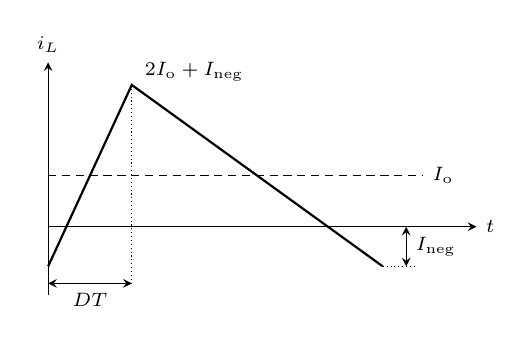
\begin{tikzpicture}[xscale=0.85, yscale=0.72, >=stealth]
					\draw[->] (0,0) -- (6.4,0) node[right, font=\scriptsize]{$t$};
					\draw[->] (0,-1.2) -- (0,2.9) node[above, font=\scriptsize]{$i_L$};
					\draw[thick] (0,-0.7) -- (1.25,2.5) -- (5,-0.7);
					\draw[densely dashed] (0,0.9) -- (5.6,0.9) node[right, font=\scriptsize]{$I_\mathrm{o}$};
					\draw[densely dotted] (1.25,2.5) -- (1.25,-1.0);
					\draw[<->] (0,-1.0) -- (1.25,-1.0) node[midway, below, font=\scriptsize]{$DT$};
					\draw[densely dotted] (5,-0.7) -- (5.5,-0.7);
					\draw[<->] (5.35,-0.7) -- (5.35,0) node[midway, right, font=\scriptsize]{$I_\mathrm{neg}$};
					\node[font=\scriptsize, anchor=south west] at (1.3,2.4) {$2I_\mathrm{o}+I_\mathrm{neg}$};
				\end{tikzpicture}
				\caption{Inductor current of a buck converter in TCM}
			\end{figure}
			\small
			\begin{equation*}
				f_\mathrm{sw}=\frac{V_\mathrm{o}\left(1-V_\mathrm{o}/V_\mathrm{in}\right)}{2L\left(I_\mathrm{o}+I_\mathrm{neg}\right)}
			\end{equation*}
		\end{column}
		\begin{column}{0.53\textwidth}
			\small
			\begin{itemize}
				\item The inductor current falls below zero in every period. The negative current $I_\mathrm{neg}$ drives the node up for ZVS of the high-side switch; the positive peak gives ZVS of the low side.
				\item $I_\mathrm{neg}$ from the energy condition: $\frac{1}{2}LI_\mathrm{neg}^2\geq Q_\mathrm{oss}(V_\mathrm{in}-2V_\mathrm{o})$.
				\item Example (B1): 48\,V to 12\,V, 100\,W, $L=225$\,nH, $I_\mathrm{neg}=1.67$\,A: 20\,A ripple at 2\,MHz. With $Q_\mathrm{oss}=10$\,nC, 1.46\,A is required.
				\item Price: $I_\mathrm{rms}=10.1$\,A instead of 8.3\,A, i.e.\ 48\,\% more conduction loss; large ripple for the inductor (L6, L7).
			\end{itemize}
		\end{column}
	\end{columns}
	\blfootnote{Sources: Erickson and Maksimovi\'c, 2020, Ch.\ 23; Tutorial 6, Task 4.}
\end{frame}

%%%%%%%%%%%%%%%%%%%%%%%%%%%%%%%%%%%%%%%%%%%%%%%%%%%%%%%%%%%%%
%% Poll: TCM frequency %%
%%%%%%%%%%%%%%%%%%%%%%%%%%%%%%%%%%%%%%%%%%%%%%%%%%%%%%%%%%%%%
% Two pages: question (page 1) and answer (page 2).
\begin{frame}<handout:1-2>
	\frametitle{TCM over the load range}
	\begin{columns}[T]
		\begin{column}{0.46\textwidth}
			\begin{figure}
				\centering
				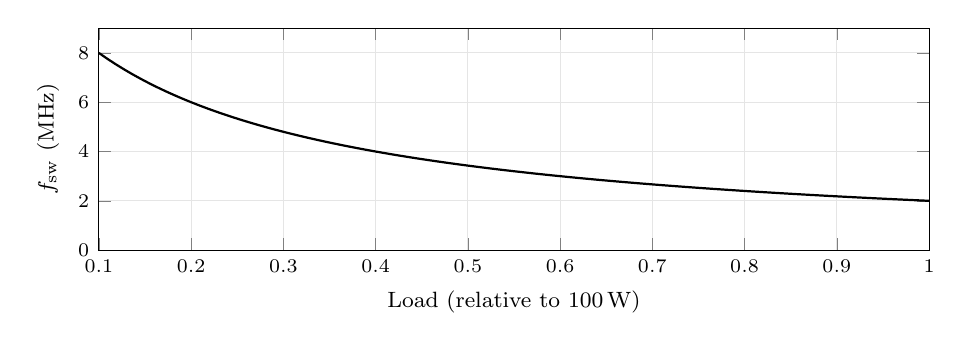
\begin{tikzpicture}
					\begin{axis}[
							width=\linewidth, height=4.4cm,
							xmin=0.1, xmax=1, ymin=0, ymax=9,
							xlabel={Load (relative to 100\,W)}, ylabel={$f_\mathrm{sw}$ (MHz)},
							grid=major, grid style={gray!20},
							tick label style={font=\scriptsize}, label style={font=\footnotesize},
						]
						\addplot[black, thick, domain=0.1:1, samples=100] {20/(8.333*x+1.667)};
					\end{axis}
				\end{tikzpicture}
				\caption{Switching frequency of the TCM example with constant $I_\mathrm{neg}=1.67$\,A}
			\end{figure}
		\end{column}
		\begin{column}{0.51\textwidth}
			\small
			Why must the frequency of a TCM converter change with the load? Discuss with your neighbour (2 minutes).
			\onslide<2-|handout:2>{
				\begin{block}{Answer}
					The current must swing from $-I_\mathrm{neg}$ to $2I_\mathrm{o}+I_\mathrm{neg}$ in every period, and the inductor voltages fix the slopes. A smaller load means a smaller swing and a shorter period: 2\,MHz at full load, 8\,MHz at 10\,\% load. At fixed frequency $I_\mathrm{neg}$ would have to grow at light load: more circulating current. Practical controllers clamp the frequency and use burst mode at light load. Interleaved phases cancel part of the large ripple at the output.
				\end{block}
			}
		\end{column}
	\end{columns}
\end{frame}

%%%%%%%%%%%%%%%%%%%%%%%%%%%%%%%%%%%%%%%%%%%%%%%%%%%%%%%%%%%%%
%% Active clamp flyback %%
%%%%%%%%%%%%%%%%%%%%%%%%%%%%%%%%%%%%%%%%%%%%%%%%%%%%%%%%%%%%%
\begin{frame}
	\frametitle{Active-clamp flyback}
	\begin{columns}[T]
		\begin{column}{0.45\textwidth}
			\begin{figure}
				\centering
				\begin{circuitikz}[scale=0.75, transform shape]
					\draw (0,0) to[V, l=$V_\mathrm{in}$] (0,5.0) -- (1.6,5.0);
					\draw (1.6,5.0) to[L, l_=$L_\mathrm{lk}$] (1.6,3.6) -- (1.6,3.3) to[L, l_=$L_\mathrm{m}$] (1.6,1.8) coordinate (d);
					\draw (1.6,5.0) -- (3.4,5.0) to[C, l=$C_\mathrm{cl}$] (3.4,3.9) -- (3.4,3.6) node[nigfete, anchor=D] (S2) {};
					\draw (S2.S) |- (d) node[circ]{};
					\draw (1.6,0) node[nigfete, anchor=S] (S1) {};
					\draw (d) -- (S1.D);
					\draw (0,0) -- (S1.S);
					\draw (0.8,0) node[ground]{};
					\node[font=\scriptsize, anchor=west] at (1.85,0.55) {$S_1$};
					\node[font=\scriptsize, anchor=west] at (3.65,2.95) {$S_2$};
					\node[font=\scriptsize, anchor=west] at (1.7,1.45) {$v_\mathrm{DS1}$};
				\end{circuitikz}
				\caption{Primary side of an active-clamp flyback (secondary not shown)}
			\end{figure}
		\end{column}
		\begin{column}{0.52\textwidth}
			\small
			\begin{itemize}
				\item The clamp capacitor and switch $S_2$ take up the leakage energy and return it, instead of burning it in an RCD clamp.
				\item Before $S_1$ turns on, $S_2$ stays on long enough for the magnetising current to become negative; this current discharges $v_\mathrm{DS1}$: ZVS of $S_1$. $S_2$ switches with ZVS as well.
				\item Controllers with adaptive ZVS and burst mode run GaN flybacks up to 1\,MHz: USB-PD adapters up to 100\,W with about 93\,\% peak efficiency.
			\end{itemize}
		\end{column}
	\end{columns}
	\blfootnote{Sources: TI UCC28780 product page and reference designs (e.g.\ 100-W USB-PD adapter).}
\end{frame}

%%%%%%%%%%%%%%%%%%%%%%%%%%%%%%%%%%%%%%%%%%%%%%%%%%%%%%%%%%%%%
%% Phase-shifted full bridge %%
%%%%%%%%%%%%%%%%%%%%%%%%%%%%%%%%%%%%%%%%%%%%%%%%%%%%%%%%%%%%%
\begin{frame}
	\frametitle{Phase-shifted full bridge}
	\begin{itemize}
		\item Both legs switch with 50\,\% duty cycle; the phase shift between the legs sets the output voltage. The transformer sees $+V_\mathrm{in}$, 0 and $-V_\mathrm{in}$.
		\item Leading leg: the reflected load current drives its transition, ZVS is easy.
		\item Lagging leg: only the energy of the leakage or series inductance drives it. ZVS is lost at light load unless $L_\mathrm{lk}$ is enlarged or the magnetising current helps.
		\item Duty-cycle loss: at the start of each power interval the leakage inductance must reverse the primary current; during this time no power is transferred. It grows with $L_\mathrm{lk}I_\mathrm{o}f_\mathrm{sw}/V_\mathrm{in}$.
		\item The leakage rings with the rectifier capacitance on the secondary: clamp or snubber needed.
	\end{itemize}
	\begin{block}{Key message}
		Every ZVS scheme borrows its energy from an inductance; where that inductance carries little current, ZVS ends.
	\end{block}
	\blfootnote{Source: Erickson and Maksimovi\'c, 3rd ed., 2020, Ch.\ 23.}
\end{frame}

%%%%%%%%%%%%%%%%%%%%%%%%%%%%%%%%%%%%%%%%%%%%%%%%%%%%%%%%%%%%%
%% DAB %%
%%%%%%%%%%%%%%%%%%%%%%%%%%%%%%%%%%%%%%%%%%%%%%%%%%%%%%%%%%%%%
\begin{frame}
	\frametitle{Dual active bridge}
	\begin{columns}[T]
		\begin{column}{0.46\textwidth}
			\begin{figure}
				\centering
				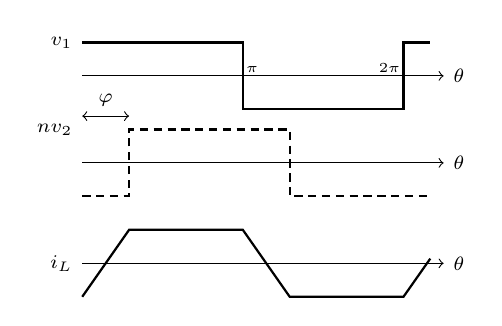
\begin{tikzpicture}[scale=0.85]
					% v1
					\draw[->] (0,2.2) -- (5.4,2.2) node[right, font=\scriptsize]{$\theta$};
					\draw[thick] (0,2.7) -- (2.4,2.7) -- (2.4,1.7) -- (4.8,1.7) -- (4.8,2.7) -- (5.2,2.7);
					\node[font=\scriptsize, anchor=east] at (0,2.7) {$v_1$};
					% v2'
					\draw[->] (0,0.9) -- (5.4,0.9) node[right, font=\scriptsize]{$\theta$};
					\draw[thick, densely dashed] (0,0.4) -- (0.7,0.4) -- (0.7,1.4) -- (3.1,1.4) -- (3.1,0.4) -- (5.2,0.4);
					\node[font=\scriptsize, anchor=east] at (0,1.4) {$nv_2$};
					\draw[<->] (0,1.6) -- (0.7,1.6) node[midway, above, font=\scriptsize]{$\varphi$};
					% iL for d = 1
					\draw[->] (0,-0.6) -- (5.4,-0.6) node[right, font=\scriptsize]{$\theta$};
					\draw[thick] (0,-1.1) -- (0.7,-0.1) -- (2.4,-0.1) -- (3.1,-1.1) -- (4.8,-1.1) -- (5.2,-0.53);
					\node[font=\scriptsize, anchor=east] at (0,-0.6) {$i_L$};
					\node[font=\tiny, anchor=south west, inner sep=1pt] at (2.4,2.2) {$\pi$};
						\node[font=\tiny, anchor=south east, inner sep=1pt] at (4.8,2.2) {$2\pi$};
				\end{tikzpicture}
				\caption{Bridge voltages and inductor current for single phase shift, $nV_2=V_1$}
			\end{figure}
		\end{column}
		\begin{column}{0.51\textwidth}
			\small
			Two full bridges, a transformer ($n$:1) and a series inductance $L$. The phase shift $\varphi$ sets the power:
			\begin{equation*}
				P=\frac{nV_1V_2\,\varphi\,(\pi-|\varphi|)}{2\pi^2f_\mathrm{sw}L}
			\end{equation*}
			\begin{itemize}
				\item Bidirectional, galvanic isolation, both bridges can switch with ZVS.
				\item Maximum at $\varphi=\pi/2$: $P_\mathrm{max}=nV_1V_2/(8f_\mathrm{sw}L)$.
				\item Example (B3): 48\,V$\leftrightarrow$12\,V, $n=4$, 1\,MHz, $L=0.8\,\mu$H: 200\,W at $\varphi=30^\circ$, $P_\mathrm{max}=360$\,W; switching currents $\pm5$\,A.
			\end{itemize}
		\end{column}
	\end{columns}
	\blfootnote{Source: De Doncker, Divan, Kheraluwala, IEEE Trans.\ Ind.\ Appl., vol.\ 27, no.\ 1, 1991.}
\end{frame}

%%%%%%%%%%%%%%%%%%%%%%%%%%%%%%%%%%%%%%%%%%%%%%%%%%%%%%%%%%%%%
%% DAB ZVS range %%
%%%%%%%%%%%%%%%%%%%%%%%%%%%%%%%%%%%%%%%%%%%%%%%%%%%%%%%%%%%%%
\begin{frame}
	\frametitle{ZVS range of the DAB}
	\begin{columns}[T]
		\begin{column}{0.48\textwidth}
			\begin{figure}
				\centering
				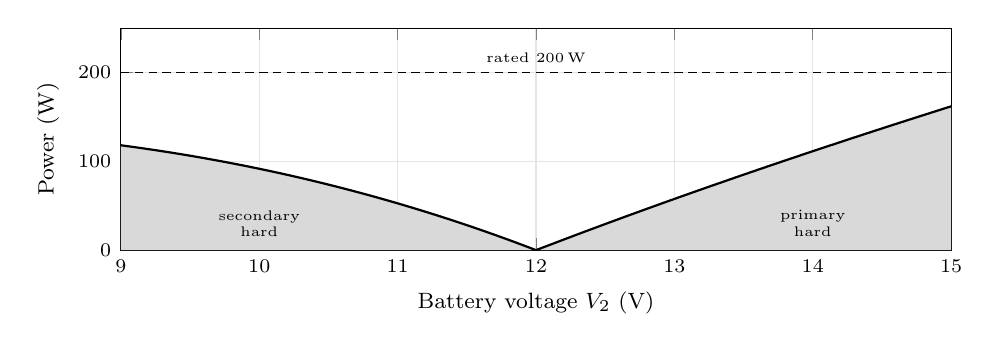
\begin{tikzpicture}
					\begin{axis}[
							width=\linewidth, height=4.4cm,
							xmin=9, xmax=15, ymin=0, ymax=250,
							xlabel={Battery voltage $V_2$ (V)}, ylabel={Power (W)},
							grid=major, grid style={gray!20},
							tick label style={font=\scriptsize}, label style={font=\footnotesize},
						]
						\addplot[fill=gray!30, draw=none, domain=9:12, samples=60] {12.159*x*(pi/2*(1-x/12))*(pi-pi/2*(1-x/12))} \closedcycle;
						\addplot[fill=gray!30, draw=none, domain=12:15, samples=60] {12.159*x*(pi/2*(1-12/x))*(pi-pi/2*(1-12/x))} \closedcycle;
						\addplot[black, thick, domain=9:12, samples=60] {12.159*x*(pi/2*(1-x/12))*(pi-pi/2*(1-x/12))};
						\addplot[black, thick, domain=12:15, samples=60] {12.159*x*(pi/2*(1-12/x))*(pi-pi/2*(1-12/x))};
						\addplot[black, densely dashed, domain=9:15, samples=2] {200};
						\node[font=\tiny, anchor=south] at (axis cs:12,200) {rated 200\,W};
						\node[font=\tiny, align=center] at (axis cs:10,30) {secondary\\hard};
						\node[font=\tiny, align=center] at (axis cs:14,30) {primary\\hard};
					\end{axis}
				\end{tikzpicture}
				\caption{B3 example; grey: one bridge loses ZVS (current sign)}
			\end{figure}
		\end{column}
		\begin{column}{0.49\textwidth}
			\small
			With the voltage ratio $d=nV_2/V_1$, the inductor current at the switching instants of the primary (0) and secondary ($\varphi$) is
			\begin{align*}
				i(0)       & =-\frac{V_1}{4f_\mathrm{sw}L}\left(1-d+\frac{2d\varphi}{\pi}\right) \\
				i(\varphi) & =\frac{V_1}{4f_\mathrm{sw}L}\left(d-1+\frac{2\varphi}{\pi}\right)
			\end{align*}
			\begin{itemize}
				\item $d=1$: ZVS of both bridges at every load.
				\item $d\neq1$: the bridge with the lower voltage loses ZVS at light load.
				\item The current sign is necessary, not sufficient: $2Q_\mathrm{oss}$ must also flow within $t_\mathrm{d}$.
			\end{itemize}
		\end{column}
	\end{columns}
	\blfootnote{Sources: De Doncker et al., 1991; Everts et al., IEEE ECCE 2013.}
\end{frame}

%%%%%%%%%%%%%%%%%%%%%%%%%%%%%%%%%%%%%%%%%%%%%%%%%%%%%%%%%%%%%
%% Think pair share: DAB light load %%
%%%%%%%%%%%%%%%%%%%%%%%%%%%%%%%%%%%%%%%%%%%%%%%%%%%%%%%%%%%%%
% Two pages: question (page 1) and answer (page 2).
\begin{frame}<handout:1-2>
	\frametitle{DAB at light load}
	\begin{block}{Think, pair, share (5 minutes)}
		The DAB of B3 ($n=4$, 1\,MHz, $L=0.8\,\mu$H) charges a battery between 10\,V and 14\,V from 48\,V.
		\begin{enumerate}
			\item Below which power does it lose ZVS at 10\,V and at 14\,V, and which bridge?
			\item Name three ways to extend the ZVS range.
		\end{enumerate}
	\end{block}
	\onslide<2-|handout:2>{
		\small
		\begin{enumerate}
			\item 10\,V: $d=0.83$, the secondary needs $\varphi>\frac{\pi}{2}(1-d)=15^\circ$, i.e.\ $P>92$\,W. 14\,V: $d=1.17$, the primary needs $\varphi>\frac{\pi}{2}(1-1/d)=12.9^\circ$, i.e.\ $P>111$\,W. About half of the rated power range is hard-switched on one side.
			\item Modulation with more degrees of freedom (duty cycles of the bridges, extended or triple phase shift; Sha and Xu, 2018), variable frequency, commutation inductances that add a reactive current (Everts et al.), a transformer ratio that matches the most frequent operating point.
		\end{enumerate}
	}
\end{frame}

%%%%%%%%%%%%%%%%%%%%%%%%%%%%%%%%%%%%%%%%%%%%%%%%%%%%%%%%%%%%%
%% Auxiliary circuits %%
%%%%%%%%%%%%%%%%%%%%%%%%%%%%%%%%%%%%%%%%%%%%%%%%%%%%%%%%%%%%%
\subsection{Auxiliary circuits and resonant switches}

\begin{frame}
	\frametitle{Auxiliary commutation circuits}
	\begin{itemize}
		\item Zero-voltage transition (ZVT): a small auxiliary switch and inductor discharge the main switch just before it turns on. The main switch is soft, the auxiliary switch carries a short current pulse (Hua, Leu, Lee, 1992).
		\item Zero-current transition (ZCT): the same idea for the turn-off of IGBTs.
		\item Auxiliary resonant commutated pole (ARCP): an auxiliary branch at the midpoint of each inverter leg for high-power inverters (De Doncker, Lyons, 1990).
		\item At MHz these schemes are rarely used: one more switch, one more gate driver, nanosecond timing. With GaN, TCM or a small negative current in the main inductor achieves the same with fewer parts.
	\end{itemize}
	\blfootnote{Sources: Hua, Leu, Lee, IEEE PESC 1992; De Doncker and Lyons, IEEE IAS Annual Meeting 1990.}
\end{frame}

%%%%%%%%%%%%%%%%%%%%%%%%%%%%%%%%%%%%%%%%%%%%%%%%%%%%%%%%%%%%%
%% Resonant switches %%
%%%%%%%%%%%%%%%%%%%%%%%%%%%%%%%%%%%%%%%%%%%%%%%%%%%%%%%%%%%%%
\begin{frame}
	\frametitle{Resonant switches}
	\begin{columns}[T]
		\begin{column}{0.52\textwidth}
			\small
			\begin{itemize}
				\item A small $L_\mathrm{r}$ and $C_\mathrm{r}$ around the switch make each switching event a short resonance: zero-current (ZCS) or zero-voltage (ZVS) quasi-resonant converters (Liu, Oruganti, Lee, 1987).
				\item ZVS quasi-resonant buck: when the switch turns off, $C_\mathrm{r}$ resonates with $L_\mathrm{r}$:
				      \begin{equation*}
					      v_\mathrm{pk}=V_\mathrm{in}+Z_0I_\mathrm{o},\qquad Z_0=\sqrt{L_\mathrm{r}/C_\mathrm{r}}
				      \end{equation*}
				      The voltage only returns to zero if $Z_0I_\mathrm{o}\geq V_\mathrm{in}$: the switch sees at least $2V_\mathrm{in}$.
			\end{itemize}
		\end{column}
		\begin{column}{0.45\textwidth}
			\small
			\textbf{Why they faded}
			\begin{itemize}
				\item The switch sees a high voltage or current stress.
				\item The output is controlled by the frequency over a wide range.
				\item ZVS holds only within a limited load range.
			\end{itemize}
			\textbf{Where the idea survives}
			\begin{itemize}
				\item Quasi-resonant flyback: turn-on in the valley of the ringing between $L_\mathrm{m}$ and $C_\mathrm{oss}$.
				\item The resonant converters of L9 and L10.
			\end{itemize}
		\end{column}
	\end{columns}
	\blfootnote{Source: K.-H. Liu, R. Oruganti, F.\,C. Lee, IEEE Trans.\ Power Electron., vol.\ 2, no.\ 1, 1987.}
\end{frame}

%%%%%%%%%%%%%%%%%%%%%%%%%%%%%%%%%%%%%%%%%%%%%%%%%%%%%%%%%%%%%
%% Modelling %%
%%%%%%%%%%%%%%%%%%%%%%%%%%%%%%%%%%%%%%%%%%%%%%%%%%%%%%%%%%%%%
\subsection{Modelling and simulation}

\begin{frame}
	\frametitle{Simulating soft-switched converters}
	\begin{columns}[T]
		\begin{column}{0.5\textwidth}
			\small
			\textbf{Piecewise-linear state space}
			\begin{equation*}
				\dot{\mathbf{x}}=\mathbf{A}_k\mathbf{x}+\mathbf{B}_k\mathbf{u}\quad\text{in interval }k
			\end{equation*}
			\begin{itemize}
				\item The sequence of intervals follows from events: gate edges, zero crossings, end of a transition.
				\item Periodic steady state directly: find $\mathbf{x}_0$ with $\mathbf{x}(T)=\mathbf{x}_0$ (shooting method), instead of simulating thousands of periods with nanosecond events.
			\end{itemize}
		\end{column}
		\begin{column}{0.47\textwidth}
			\small
			\textbf{Why averaging fails}
			\begin{itemize}
				\item Averaged models assume a small ripple and a fixed period. In TCM the ripple is larger than the DC current and the period changes with the load.
				\item Sampled-data model: $\mathbf{x}[k+1]=\mathbf{f}(\mathbf{x}[k],\mathbf{u}[k])$, linearised to $\tilde{\mathbf{x}}[k+1]=\boldsymbol{\Phi}\tilde{\mathbf{x}}[k]+\boldsymbol{\Gamma}\tilde{\mathbf{u}}[k]$: exact at the sampling instants, and directly a $z$-domain model for digital control (L13).
			\end{itemize}
		\end{column}
	\end{columns}
	\blfootnote{Sources: Maksimovi\'c and Zane, IEEE TPEL, vol.\ 22, no.\ 6, 2007; Corradini, Maksimovi\'c, Mattavelli, Zane, \textit{Digital Control of High-Frequency Switched-Mode Power Converters}, Wiley, 2015.}
\end{frame}

%%%%%%%%%%%%%%%%%%%%%%%%%%%%%%%%%%%%%%%%%%%%%%%%%%%%%%%%%%%%%
%% Live simulation %%
%%%%%%%%%%%%%%%%%%%%%%%%%%%%%%%%%%%%%%%%%%%%%%%%%%%%%%%%%%%%%
\begin{frame}
	\frametitle{Hard or soft: simulation}
	\begin{columns}[T]
		\begin{column}{0.5\textwidth}
			\textbf{Demonstration} (\texttt{lecture/sim/zvs\_halfbridge.cir}, ngspice)
			\begin{enumerate}
				\item Half-bridge at 48\,V, $Q_\mathrm{oss}=10$\,nC, 200\,nH, dead time 12\,ns.
				\item Case A: $I_0=+3$\,A into the node.
				\item Case B: $I_0=-3$\,A.
				\item Change the dead time to 5\,ns.
			\end{enumerate}
		\end{column}
		\begin{column}{0.47\textwidth}
			\textbf{Observe}
			\begin{itemize}
				\item A: the node reaches 48\,V after 7.5\,ns; for the rest of the dead time the high side conducts in reverse. Turn-on energy 2\,nJ.
				\item B: the low side conducts in reverse at $-1.9$\,V; hard turn-on with 0.56\,$\mu$J ($Q_\mathrm{oss}V=0.48\,\mu$J plus overlap), 1.1\,W at 2\,MHz.
				\item 5\,ns: turn-on at about 30\,V, 63\,nJ.
			\end{itemize}
		\end{column}
	\end{columns}
\end{frame}

%%%%%%%%%%%%%%%%%%%%%%%%%%%%%%%%%%%%%%%%%%%%%%%%%%%%%%%%%%%%%
%% Checklist %%
%%%%%%%%%%%%%%%%%%%%%%%%%%%%%%%%%%%%%%%%%%%%%%%%%%%%%%%%%%%%%
\subsection{Design for ZVS}

\begin{frame}
	\frametitle{ZVS design checklist}
	\begin{columns}[T]
		\begin{column}{0.5\textwidth}
			\small
			\textbf{At every switching instant, over load and line}
			\begin{enumerate}
				\item Current direction towards the next conducting switch.
				\item Charge: $2Q_\mathrm{oss}$ plus transformer and winding capacitance within $t_\mathrm{d}$.
				\item Energy: $\frac{1}{2}LI^2\geq Q_\mathrm{oss}(V-2V_x)$ when the current is not stiff.
				\item Margins: $C_\mathrm{oss}$ tolerance, temperature, layout capacitance of the switch node.
				\item Dead time adapted to the current (L4).
			\end{enumerate}
		\end{column}
		\begin{column}{0.47\textwidth}
			\small
			\textbf{What ZVS does not remove}
			\begin{itemize}
				\item $C_\mathrm{oss}$ hysteresis loss (L2, L5)
				\item turn-off overlap (small with fast turn-off and $C_\mathrm{oss}$ as snubber)
				\item gate loss and dead-time conduction
				\item the larger RMS current
			\end{itemize}
			\begin{block}{Key message}
				ZVS is designed at the worst operating point, usually light load.
			\end{block}
		\end{column}
	\end{columns}
\end{frame}

%%%%%%%%%%%%%%%%%%%%%%%%%%%%%%%%%%%%%%%%%%%%%%%%%%%%%%%%%%%%%
%% Soft switching in the briefs %%
%%%%%%%%%%%%%%%%%%%%%%%%%%%%%%%%%%%%%%%%%%%%%%%%%%%%%%%%%%%%%
\begin{frame}
	\frametitle{Soft switching in the briefs}
	\begin{table}
		\centering
		\footnotesize
		\begin{tabular}{|l|>{\raggedright\arraybackslash}p{3.0cm}|>{\raggedright\arraybackslash}p{9.6cm}|}
			\hline
			   & \textbf{Brief}           & \textbf{ZVS question}                                                                                         \\
			\hline
			B1 & ZVS GaN buck, 1--3\,MHz  & $I_\mathrm{neg}$ from the energy condition; frequency range, clamp and burst at light load; dead time        \\
			B2 & LLC DCX, 1\,MHz          & magnetising current and dead time deliver $2Q_\mathrm{oss}$ (L9)                                              \\
			B3 & DAB, 0.5--1\,MHz         & ZVS boundaries over the battery voltage; modulation that extends them                                        \\
			B4 & 6.78\,MHz class E        & ZVS and zero $\mathrm{d}v/\mathrm{d}t$ by the load network; sensitivity to the coil position (L10)            \\
			B5 & 13.56\,MHz VHF           & ZVS with $C_\mathrm{oss}$ inside the tank (L10)                                                               \\
			B6 & hybrid SC, 48\,V         & soft charging and ZVS of the flying-capacitor switches (L12)                                                  \\
			\hline
		\end{tabular}
		\caption{Milestone M2 (16.12., PDR): ZVS checked at the worst-case operating points}
	\end{table}
\end{frame}

%%%%%%%%%%%%%%%%%%%%%%%%%%%%%%%%%%%%%%%%%%%%%%%%%%%%%%%%%%%%%
%% Key messages %%
%%%%%%%%%%%%%%%%%%%%%%%%%%%%%%%%%%%%%%%%%%%%%%%%%%%%%%%%%%%%%
\begin{frame}
	\frametitle{Key messages}
	\begin{enumerate}
		\item ZVS needs the right current direction, the charge $2Q_\mathrm{oss}$ within the dead time and, for a soft current, the energy $Q_\mathrm{oss}(V-2V_x)$.
		\item Energy estimates with $2E_\mathrm{oss}$ are optimistic; the charge-based value holds for any $C_\mathrm{oss}(v)$.
		\item TCM gives ZVS to a buck or boost converter at the price of RMS current and a load-dependent frequency.
		\item Active-clamp flyback, phase-shifted full bridge and DAB take the ZVS energy from leakage or magnetising inductance; they lose ZVS at light load.
		\item A DAB keeps ZVS at all loads only for $nV_2=V_1$; otherwise modulation must help.
		\item Soft-switched converters are simulated piecewise and modelled in discrete time, not with averaged models.
	\end{enumerate}
\end{frame}

%%%%%%%%%%%%%%%%%%%%%%%%%%%%%%%%%%%%%%%%%%%%%%%%%%%%%%%%%%%%%
%% Exit ticket %%
%%%%%%%%%%%%%%%%%%%%%%%%%%%%%%%%%%%%%%%%%%%%%%%%%%%%%%%%%%%%%
% Two pages: questions (page 1) and answers (page 2).
\begin{frame}<handout:1-2>
	\frametitle{Exit questions}
	\begin{varblock}[\textwidth]{Three questions, one minute each}
		\begin{enumerate}
			\item A transistor has $Q_\mathrm{oss}=25$\,nC at 48\,V. Which dead time does a stiff current of 5\,A need?
			\item Why does an LLC half-bridge, whose inductor ends at the midpoint, need no energy for the transition, but still a minimum current?
			\item A TCM buck runs at 2\,MHz at full load. Why does its efficiency drop at 10\,\% load?
		\end{enumerate}
	\end{varblock}
	\onslide<2-|handout:2>{
		\begin{enumerate}
			\item $t_\mathrm{d}\geq2\cdot25\,\mathrm{nC}/5\,\mathrm{A}=10$\,ns.
			\item With $V_x=V/2$ the inductor gains energy in the first half and returns it in the second. The charge $2Q_\mathrm{oss}$ must still flow within the dead time: $I\geq2Q_\mathrm{oss}/t_\mathrm{d}$.
			\item The frequency rises to 8\,MHz, so all frequency-proportional losses (gate, core, $C_\mathrm{oss}$ hysteresis, dead time) grow, and the RMS current is twice the load current.
		\end{enumerate}
	}
\end{frame}

%%%%%%%%%%%%%%%%%%%%%%%%%%%%%%%%%%%%%%%%%%%%%%%%%%%%%%%%%%%%%
%% References %%
%%%%%%%%%%%%%%%%%%%%%%%%%%%%%%%%%%%%%%%%%%%%%%%%%%%%%%%%%%%%%
\begin{frame}
	\frametitle{References}
	\scriptsize
	\begin{itemize}
		\item R.\,W. Erickson, D. Maksimovi\'c, \textit{Fundamentals of Power Electronics}, 3rd ed., Springer, 2020, Ch.\ 23.
		\item J.\,G. Kassakian, D.\,J. Perreault, G.\,C. Verghese, M.\,F. Schlecht, \textit{Principles of Power Electronics}, 2nd ed., Cambridge University Press, 2023.
		\item J. Everts, F. Krismer, J. Van den Keybus, J. Driesen, J.\,W. Kolar, ``Charge-based ZVS soft switching analysis of a single-stage dual active bridge AC--DC converter,'' IEEE ECCE 2013, pp.\ 4820--4829.
		\item R.\,W. De Doncker, D.\,M. Divan, M.\,H. Kheraluwala, ``A three-phase soft-switched high-power-density dc/dc converter for high-power applications,'' IEEE Trans.\ Ind.\ Appl., vol.\ 27, no.\ 1, pp.\ 63--73, 1991.
		\item D. Sha, G. Xu, \textit{High-Frequency Isolated Bidirectional Dual Active Bridge DC--DC Converters with Wide Voltage Gain}, Springer, 2018.
		\item K.-H. Liu, R. Oruganti, F.\,C. Lee, ``Quasi-resonant converters -- topologies and characteristics,'' IEEE Trans.\ Power Electron., vol.\ 2, no.\ 1, pp.\ 62--71, 1987.
	\end{itemize}
\end{frame}

\begin{frame}
	\frametitle{References (cont.)}
	\scriptsize
	\begin{itemize}
		\item G. Hua, C.-S. Leu, F.\,C. Lee, ``Novel zero-voltage-transition PWM converters,'' IEEE PESC 1992.
		\item R.\,W. De Doncker, J.\,P. Lyons, ``The auxiliary resonant commutated pole converter,'' IEEE IAS Annual Meeting, 1990, pp.\ 1228--1235.
		\item D. Maksimovi\'c, R. Zane, ``Small-signal discrete-time modeling of digitally controlled PWM converters,'' IEEE Trans.\ Power Electron., vol.\ 22, no.\ 6, pp.\ 2552--2556, 2007.
		\item L. Corradini, D. Maksimovi\'c, P. Mattavelli, R. Zane, \textit{Digital Control of High-Frequency Switched-Mode Power Converters}, Wiley, 2015.
		\item Texas Instruments, UCC28780 high-frequency active-clamp flyback controller, product page and reference designs.
	\end{itemize}
\end{frame}
